\section{Inférence de représentations structurelles décorrélées}
\label{sec:debiaisage_structurel}

Le constat de redondance informationnelle établi au chapitre précédent met en évidence une limite majeure de l'état de l'art : la difficulté des algorithmes classiques à isoler des facteurs d'influence uniques. Dans l'objectif d'offrir de meilleures perspectives d'explicabilité, ce chapitre introduit deux contributions dédiées à l'inférence de caractéristiques débiaisées, visant à purger les métriques d'une composante déjà identifiée, et en l'occurence de leur composante spatiale.

\subsection{Communautés de Louvain spatialement décorrélées}

La détection de communautés via l'algorithme de Louvain classique \cite{louvain2008}, s'appuie nativement sur le modèle nul de configuration de Newman-Girvan. Ce modèle souffre d'une faiblesse théorique : il suppose que la probabilité de connexion entre deux nœuds ne dépend que de leurs degrés, ignorant toute autre contrainte telle que la distance physique par exemple. En présence d'un réseau hybride géométrico-communautaire, Louvain interprète mécaniquement le regroupement géographique de noeuds interconnectés comme une communauté topologique, créant le biais de confusion observé.

\subsubsection{Inférence du modèle nul gravitaire}
Pour lever ce verrou, l'approche présentée s'inspire directement des travaux de Cazabet et al. \cite{cazabet2022enhancing}, qui injectent un modèle nul spatial contraint par les degrés ($\text{DC-Spatial}$) directement au cœur du critère d'optimisation de l'algorithme de Louvain. La spécificité de la méthode proposée est que le Null Modèle spatial utilisé est directement inféré à partir du graphe étudié lui même.
Pour cela, nous inférons un modèle gravitaire dont la probabilité d'existence d'un lien est gouvernée par des potentiels de nœuds $\alpha$ (degrés latents) et un paramètre d'échelle global $\beta$ pondérant l'impact de la distance sur la connexion des noeuds. La matrice de probabilité du modèle nul $P$ est inférée par maximum de vraisemblance via un algorithme itératif de descente de coordonnées, combiné à une méthode de Newton :

\begin{equation}
    P_{uv} = \frac{1}{1 + e^{-(\alpha_u + \alpha_v - \beta \cdot d_{uv})}}
\end{equation}

Les paramètres nodaux $\alpha$ ajustent la contrainte sur les degrés attendus, tandis que l'optimisation scalaire de $\beta$ maximise la log-vraisemblance globale sur le triangle supérieur de la matrice d'adjacence $A$. Pour garantir la symétrie stricte exigée par le calcul de modularité, la matrice finale du modèle nul est définie par $P^{\text{sym}} = (P + P^T)/2$.

\subsubsection{Optimisation de la modularité ignorant l'influence spatiale}

Cette matrice $P^{\text{sym}}$ est ensuite substituée au modèle nul classique au sein de l'algorithme \texttt{MetaLouvain}, développé dans les travaux de Rémy Cazabet. La nouvelle fonction de modularité modifiée évalue l'écart entre la topologie observée et les prédictions du modèle nul gravitaire où $A_{uv}$ désigne un élément de la matrice d'adjacence du réseau, et $b_u$ et $b_v$ les identifiants des communautés respectives des nœuds $u$ et $v$~:

\begin{equation}
\label{eq:q_spatial}
    Q_{\text{Spatial}} = \frac{1}{2m} \sum_{u,v} \left( A_{uv} - P^{\text{sym}}_{uv} \right) \mathbb{I}(b_u = b_v)
\end{equation}

En soustrayant la probabilité de liaison capturée par le modèle nul géométrique, le modèle ne considère comme significatives que les arêtes qui s'établissent au-delà des attentes gravitaires. Les communautés ainsi extraites découlent d'un signal d'affinité topologique pure (et de résidus statistiques, ou bruit), purgé de l'effet de proximité géographique dans la mesure de ce que le modèle nul parvient à capturer.


\subsection{Plongements géométriques type SiNE spatialement décorrélés}

Si l'approche précédente montre des résultats intéressants (voir partie \ref{sec:5_3Validafion}), elle se heurte à une faiblesse intrinsèque des algorithmes de partitionnement : le besoin d'un fort signal de densité pour converger vers des blocs stables. Pour capturer des signaux d'affinité plus diffus, nous basculons vers une nouvelle approche en transposant le concept de décorrélation au sein des plongements de graphes (\textit{graph embeddings}).

\subsubsection{Formulation de la matrice de résidus}
Plutôt que d'apprendre des représentations sur la matrice d'adjacence brute $A$, notre méthode, baptisée $\text{SiNE décorrelée}$, opère sur la \textbf{matrice de résidus} structurels $R$, définie par la soustraction du modèle nul gravitaire inféré précédemment :
\begin{equation}
    R = A - P^{\text{sym}}
\end{equation}
Cette opération transforme le réseau en un graphe signé virtuel où $R_{uv} \ge 0$ traduit une sur-représentation topologique (affinité positive) et $R_{uv} < 0$ une sous-représentation (répulsion négative) par rapport à la contrainte spatiale.

\subsubsection{Échantillonnage stochastique par Softmax}
Pour guider l'apprentissage, nous implémentons un protocole d'échantillonnage de paires dyadiques basé sur l'intensité des résidus. Pour chaque nœud $i$, les candidats valides font l'objet d'un tirage aléatoire sans remise pondéré par une distribution Softmax appliquée sur la valeur absolue des résidus $|R_{ij}|$, modulée par un paramètre de température $T$ :
\begin{equation}
    p(j \mid i) = \frac{e^{|R_{ij}| / T}}{\sum_{w \in \mathcal{V}_i} e^{|R_{iw}| / T}}
\end{equation}
Ce mécanisme force l'algorithme à focaliser son attention sur les dyades qui manifestent les plus fortes déviations (positives ou négatives) vis-à-vis du modèle nul.

\subsubsection{Optimisation par perte de signe paire-à-paire} La complexité de la méthode réside dans le fait d'avoir à gérer des pondérations de liens positives comme négatives. Pour résoudre ce problème, les plongements continus en dimension $d=64$ sont optimisés de bout en bout via une fonction de perte antagoniste signée (\textit{Pairwise Sign Loss}) entraînée par l'optimisateur Adam (mécanisme inspiré des travaux de Daokun Zhang et al. \cite{wang2017SINE}). Soit $\mathbf{z}_u$ le vecteur latent du nœud $u$, la fonction de coût minimise la distance euclidienne pour les résidus positifs et applique une marge de séparation stricte ($m=2,0$) pour les résidus négatifs :
\begin{equation}
    \mathcal{L} = \mathbb{E}_{(u,v) \sim \mathcal{S}} \left[ \mathbb{I}(R_{uv} \ge 0) \|\mathbf{z}_u - \mathbf{z}_v\|_2 + \mathbb{I}(R_{uv} < 0) \max\left(0, m - \|\mathbf{z}_u - \mathbf{z}_v\|_2\right) \right]
\end{equation}

\subsection{Validation des résultats et analyse et performances empiriques}
\label{sec:5_3Validafion}

\subsubsection{Validation du fonctionnement des algorithmes}

La validation des méthodes proposées repose, dans un premier temps, sur l'évaluation de l'indépendance statistique entre les partitions et représentations latentes obtenues, vis-à-vis de la vérité terrain $\text{GT\_pos}$ par rapport à laquelle elles ont été décorrélées.

\begin{figure}
\includegraphics[width=\textwidth]{Plots/207 02_Correl_All_SBM_and_POS.png}
\caption{Evolution du coefficient de spearman entre chaque feature standard et débiaisée, et la \textit{Ground Truth} communautaire (à droite), ou la \textit{Ground Truth} géométrique (à gauche) en fonction de $\alpha$ (moyenne sur 10 itérations).} 
\label{fig6}
\end{figure}

\begin{figure}
\includegraphics[width=\textwidth]{Plots/208 02_MI_adjusted_All.png}
\caption{Evolution de l'Information Mutuelle Ajustée (AMI) entre chauque features standard et débiaisée, et la \textit{Ground Truth} communautaire (à droite), ou la \textit{Ground Truth} géométrique (à gauche) en fonction de $\alpha$ (moyenne sur 10 itérations).} 
\label{fig8}
\end{figure}

L'analyse des corrélations de Spearman (Figure \ref{fig6}) et de l'Information Mutuelle Ajustée (Figure \ref{fig8}) confirme que l'algorithme de Louvain décorrélé remplit pleinement ses objectifs théoriques. En effet, nous observons une corrélation quasi-nulle avec la vérité terrain spatiale ($\text{GT\_pos}$) sur la quasi-totalité des ratios d'hybridation $\alpha$. Une légère augmentation de cette corrélation est perceptible uniquement autour du point extrême $\alpha = 0$, configuration où l'information spatiale constitue l'unique source de structure du réseau. De plus, la corrélation et l'information mutuelle capturées avec la structure communautaire cible ($\text{GT\_sbm}$) sont améliorées sur la plage intermédiaire $0.2 \le \alpha \le 0.5$.

Des tendances similaires sont observées pour les plongements (\textit{embeddings}) issus de $\text{SiNE}$ décorrélé. Ces derniers présentent une corrélation et une quantité d'information mutuelle plus faibles avec la composante spatiale $\text{GT\_pos}$ que les plongements de référence générés par la méthode classique DeepWalk, et ce pour l'ensemble des valeurs de $\alpha$. Par ailleurs, le mécanisme de décorrélation permet à la méthode proposée de s'aligner plus fidèlement sur la structure $\text{GT\_sbm}$ de par une plus haute corrélation, sans pour autant capturer plus d'information mutuelle.

Ces premières observations valident empiriquement le comportement de nos deux approches : elles permettent d'inférer des structures communautaires (pour Louvain décorrélé) et des représentations vectorielles (pour SiNE décorrélé) significativement plus orthogonales à la topologie spatiale que les méthodes standards de la littérature.

\subsubsection{Performance des algorithmes par rapport à l'état de l'art}

Dans un second temps, afin d'évaluer la pertinence et l'apport applicatif de ces approches débiaisées, nous mesurons leurs performances dans une tâche de prédiction de liens. L'objectif est de comparer l'efficacité de l'association des descripteurs décorrélés avec la \textit{Ground Truth} spatiale ($\text{GT\_pos}$ + métrique décorrélée) face à celles des standards de l'état de l'art ($\text{GT\_pos}$ + Louvain classique, ou $\text{GT\_pos}$ + DeepWalk). Cette évaluation permet de vérifier si l'extraction d'une information plus orthogonale offre une meilleure complémentarité, et donc une meilleure compréhension de la topologie globale du graphe.

Sur les graphes générés par une hybridation par somme pondérée, les performances entre le modèle de base ($\text{GT\_pos} + \text{Louvain standard}$) et notre variante débiaisée ($\text{GT\_pos} + \text{Louvain décorrélé}$) s'avèrent très proches (Figure \ref{fig:10.1}). Néanmoins, une amélioration statistiquement significative (évaluée sur 30 itérations avec un intervalle de confiance à $95\,\%$) émerge précisément au point critique $\alpha = 0.5$. Cette zone correspond au point de transition où le conflit d'information entre géométrie et communautés est maximal, démontrant l'intérêt de la décorrélation lorsque les signaux sont très entremêlés. Sur le reste du spectre de $\alpha$, la méthode débiaisée fait jeu égal avec la référence.

Cette dynamique se confirme, de manière plus marquée, sur les graphes hybridés par la méthode dite "exposant" (Figure \ref{fig:10.2}). Cette hybridation génère des structures plus contrastées où l'apport de chaque composante est plus net. Dans cette configuration, l'approche décorrélée surclasse de manière significative l'état de l'art sur une large plage de ratios, pour $0.3 \le \alpha \le 0.7$.

Les performances sur les mêmes setups de SiNEcustom en prédiction de liens, donnent des résultats encore plus encourageants : SiNE custom + GT\_pos bat deepwalk + GT\_pos pour les aplhas entre 0.5 et 1.0, avec le plus gros écart sur 0.7, sur les hybrides par somme (Figure \ref{fig:10.3}). ET sur les hybrides par méthode exposant, ils font mieux dès 0.2 jusqu'à 1.0. On pourrait aussi dire 2-3 trucs sur la forme des courbes, mais un peu osef pour notre problématique.


Enfin, les évaluations menées sur l'algorithme $\text{SiNE}$ décorrélé révèlent des résultats encore plus prometteurs. Pour les graphes hybridés par somme (Figure \ref{fig:10.3}), la combinaison $\text{SiNE décorrélé} + \text{GT\_pos}$ surclasse le couple $\text{DeepWalk} + \text{GT\_pos}$ sur l'intervalle $0.5 \le \alpha \le 1.0$, l'écart de performance maximal étant atteint pour $\alpha = 0.7$. Enfin, sur les variantes de graphes par exposant (Figure \ref{fig:10.4}), la méthode proposée surpasse la référence sur la quasi-totalité des hybrides, dès le seuil de $\alpha = 0.2$ et jusqu'à $\alpha = 1.0$.


\begin{figure}[htbp]
    \centering
    % --- Première ligne (Plots côte à côte) ---
    \begin{minipage}[b]{0.48\textwidth}
        \centering
        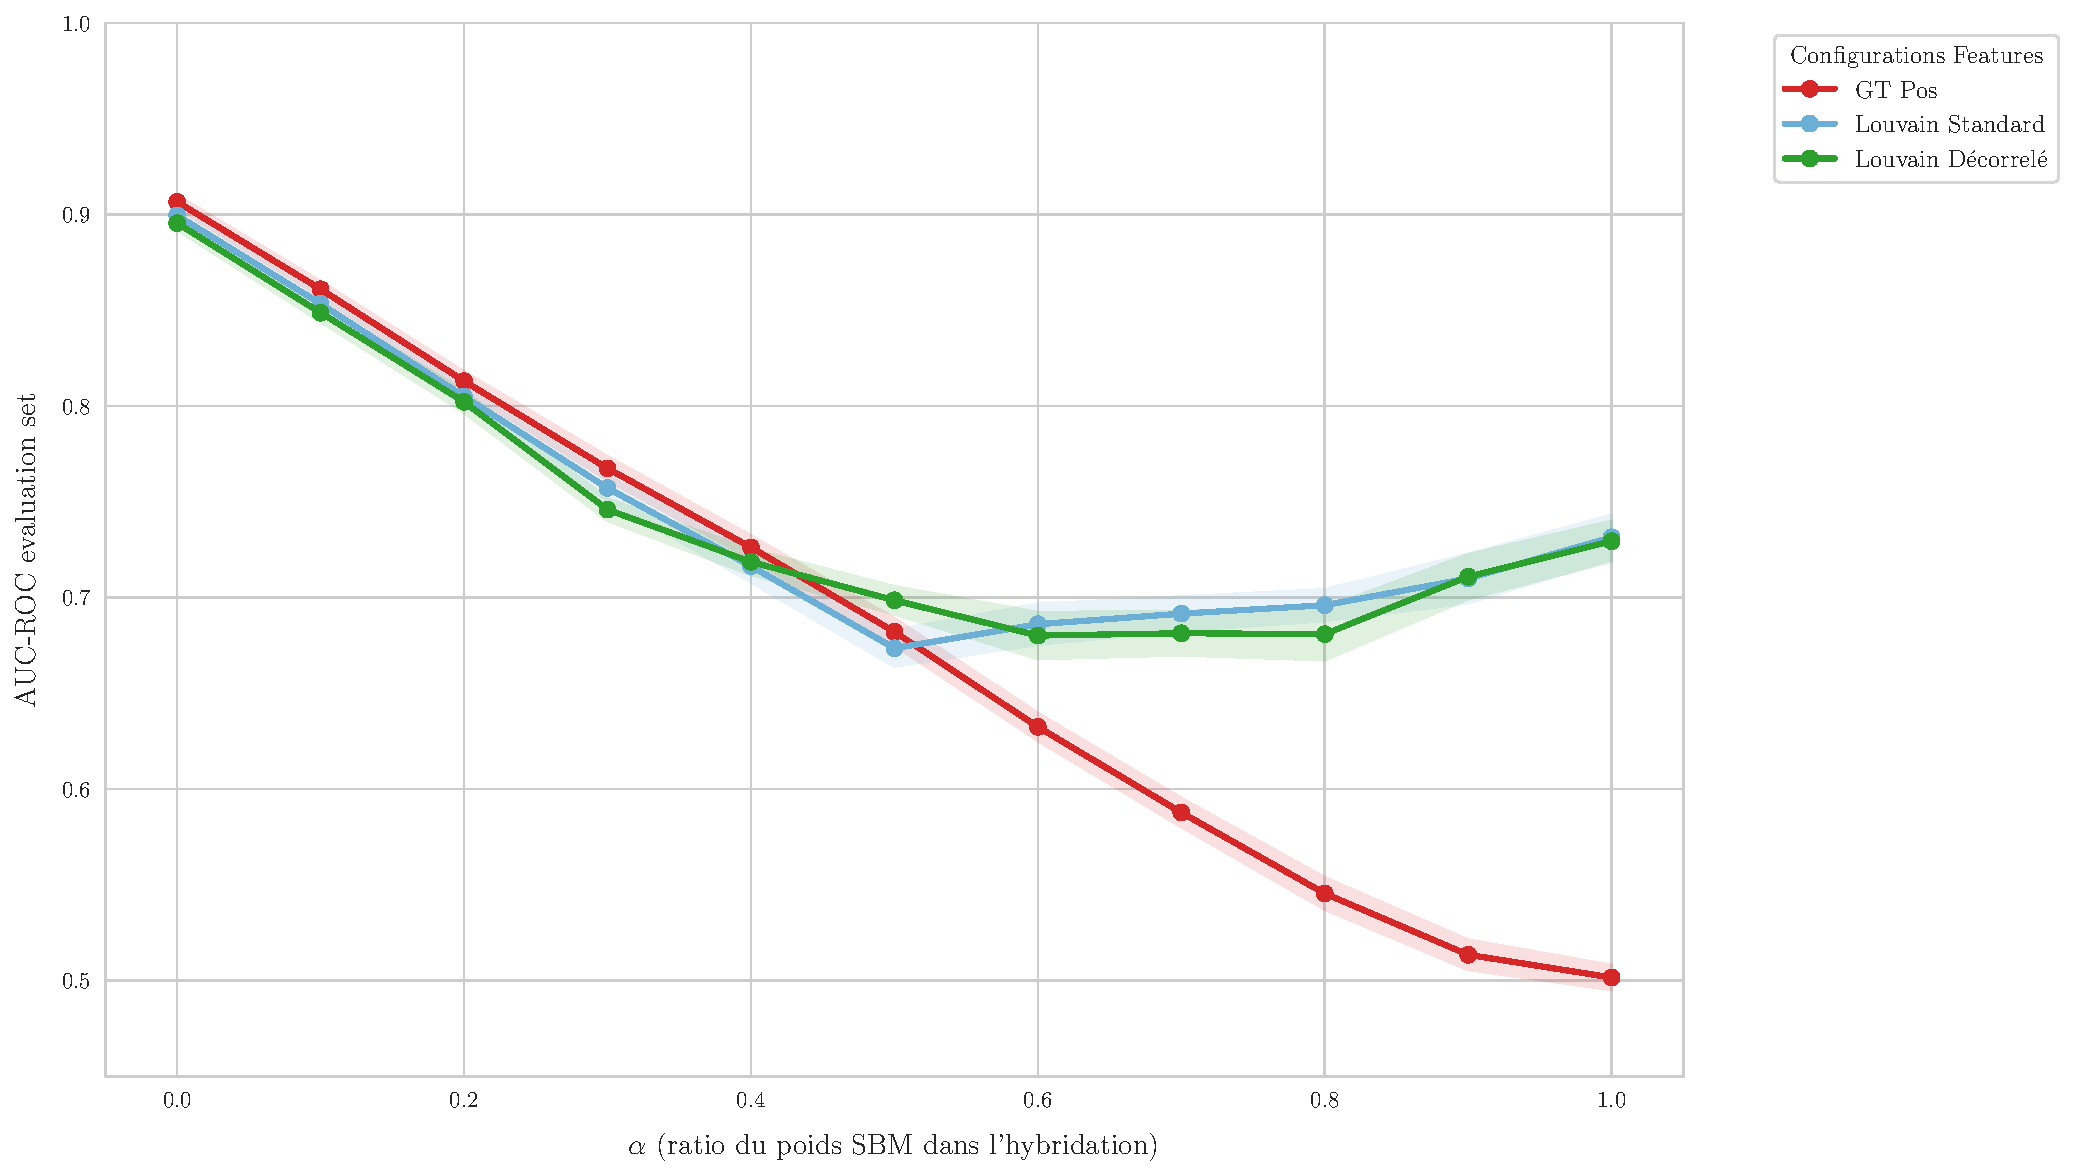
\includegraphics[width=\textwidth]{Plots/209 01_artificial_graphs_shuffled_v4_comuAndEmb_30iter_GTposAndComu_20260529_AUC-ROC_eval_CI99_SBM_ratio.pdf}
        \caption{(a) Louvain Standard vs Décorrelé (hybridation par somme pondérée)}
        \label{fig:10.1}
    \end{minipage}
    \hfill
    \begin{minipage}[b]{0.48\textwidth}
        \centering
        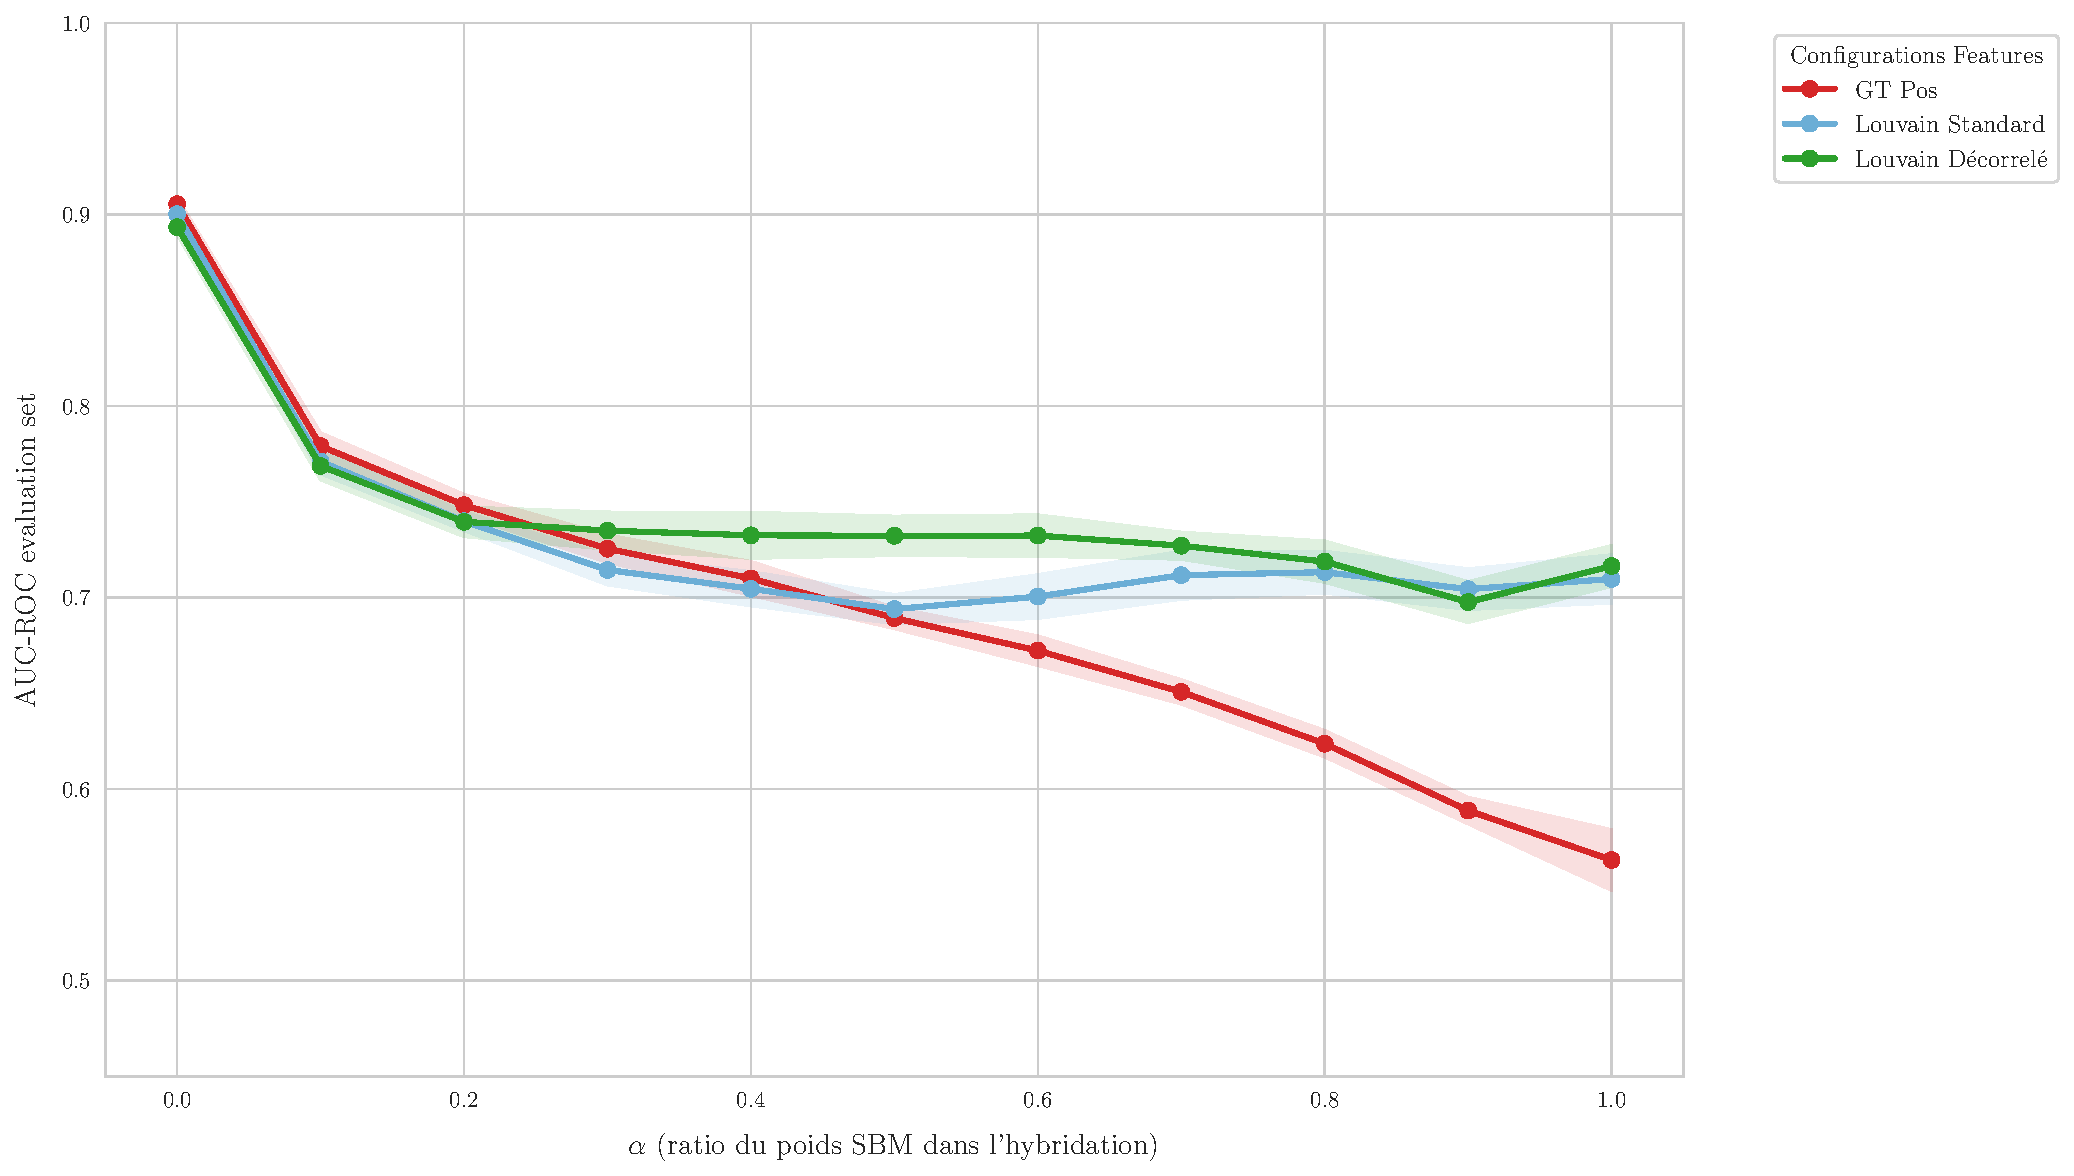
\includegraphics[width=\textwidth]{Plots/211 01_artificial_graphs_shuffled_v6_comuAndEmb_30iter_GTposAndComu_20260529_AUC-ROC_eval_CI99_SBM_ratio.pdf}
        \caption{(b) Louvain Standard vs Décorrelé (hybridation exponentielle)}
        \label{fig:10.2}
    \end{minipage}

    \vspace{0.5cm} % Espace vertical entre les deux lignes

    % --- Deuxième ligne (Plots côte à côte) ---
    \begin{minipage}[b]{0.48\textwidth}
        \centering
        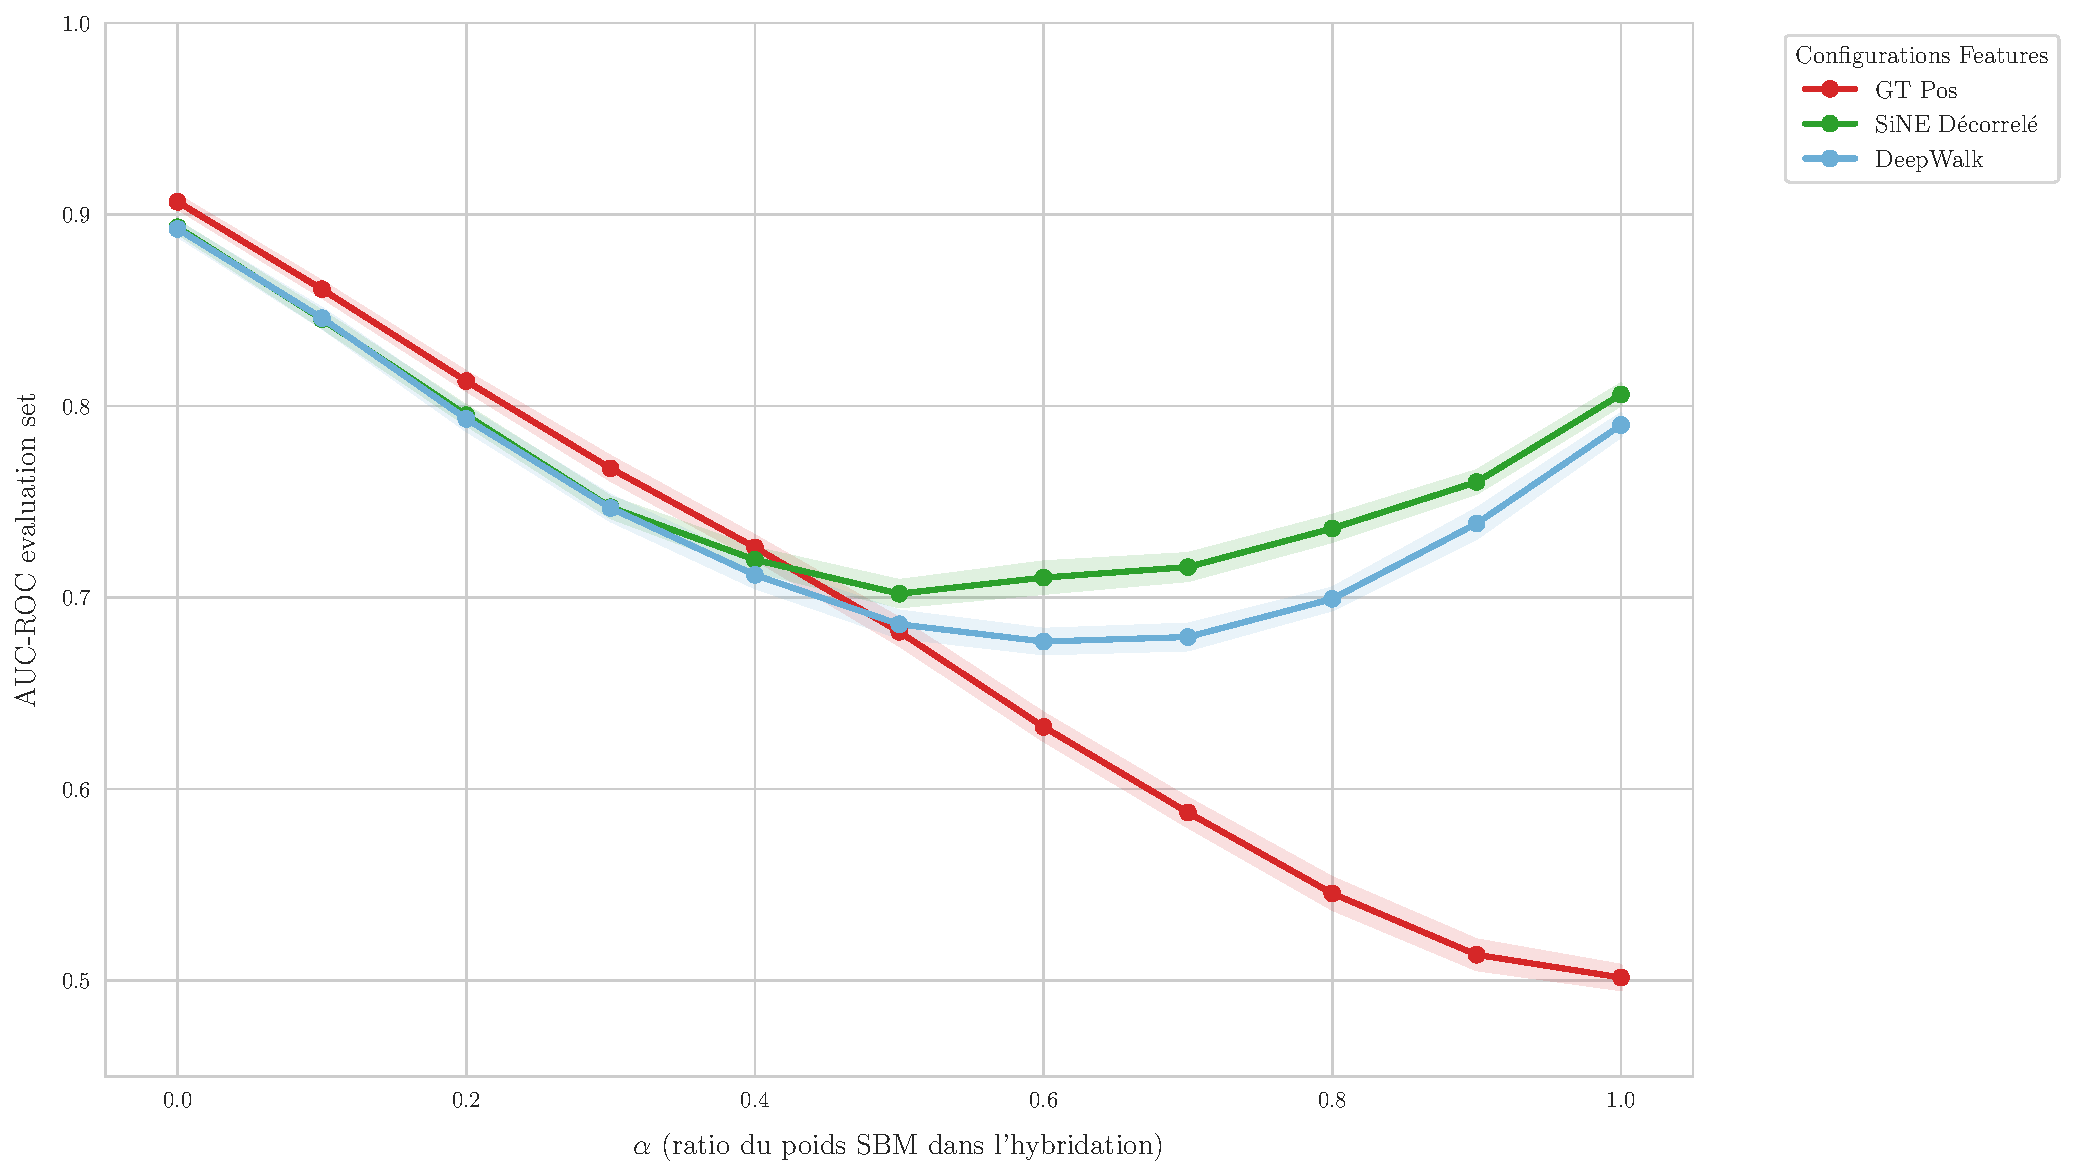
\includegraphics[width=\textwidth]{Plots/210 01_artificial_graphs_shuffled_v4_comuAndEmb_30iter_GTposAndSine_20260529_AUC-ROC_eval_CI99_SBM_ratio.pdf}
        \caption{(c) DeepWalk vs SiNE Décorrélée (hyb. par somme pondérée)}
        \label{fig:10.3}
    \end{minipage}
    \hfill
    \begin{minipage}[b]{0.48\textwidth}
        \centering
        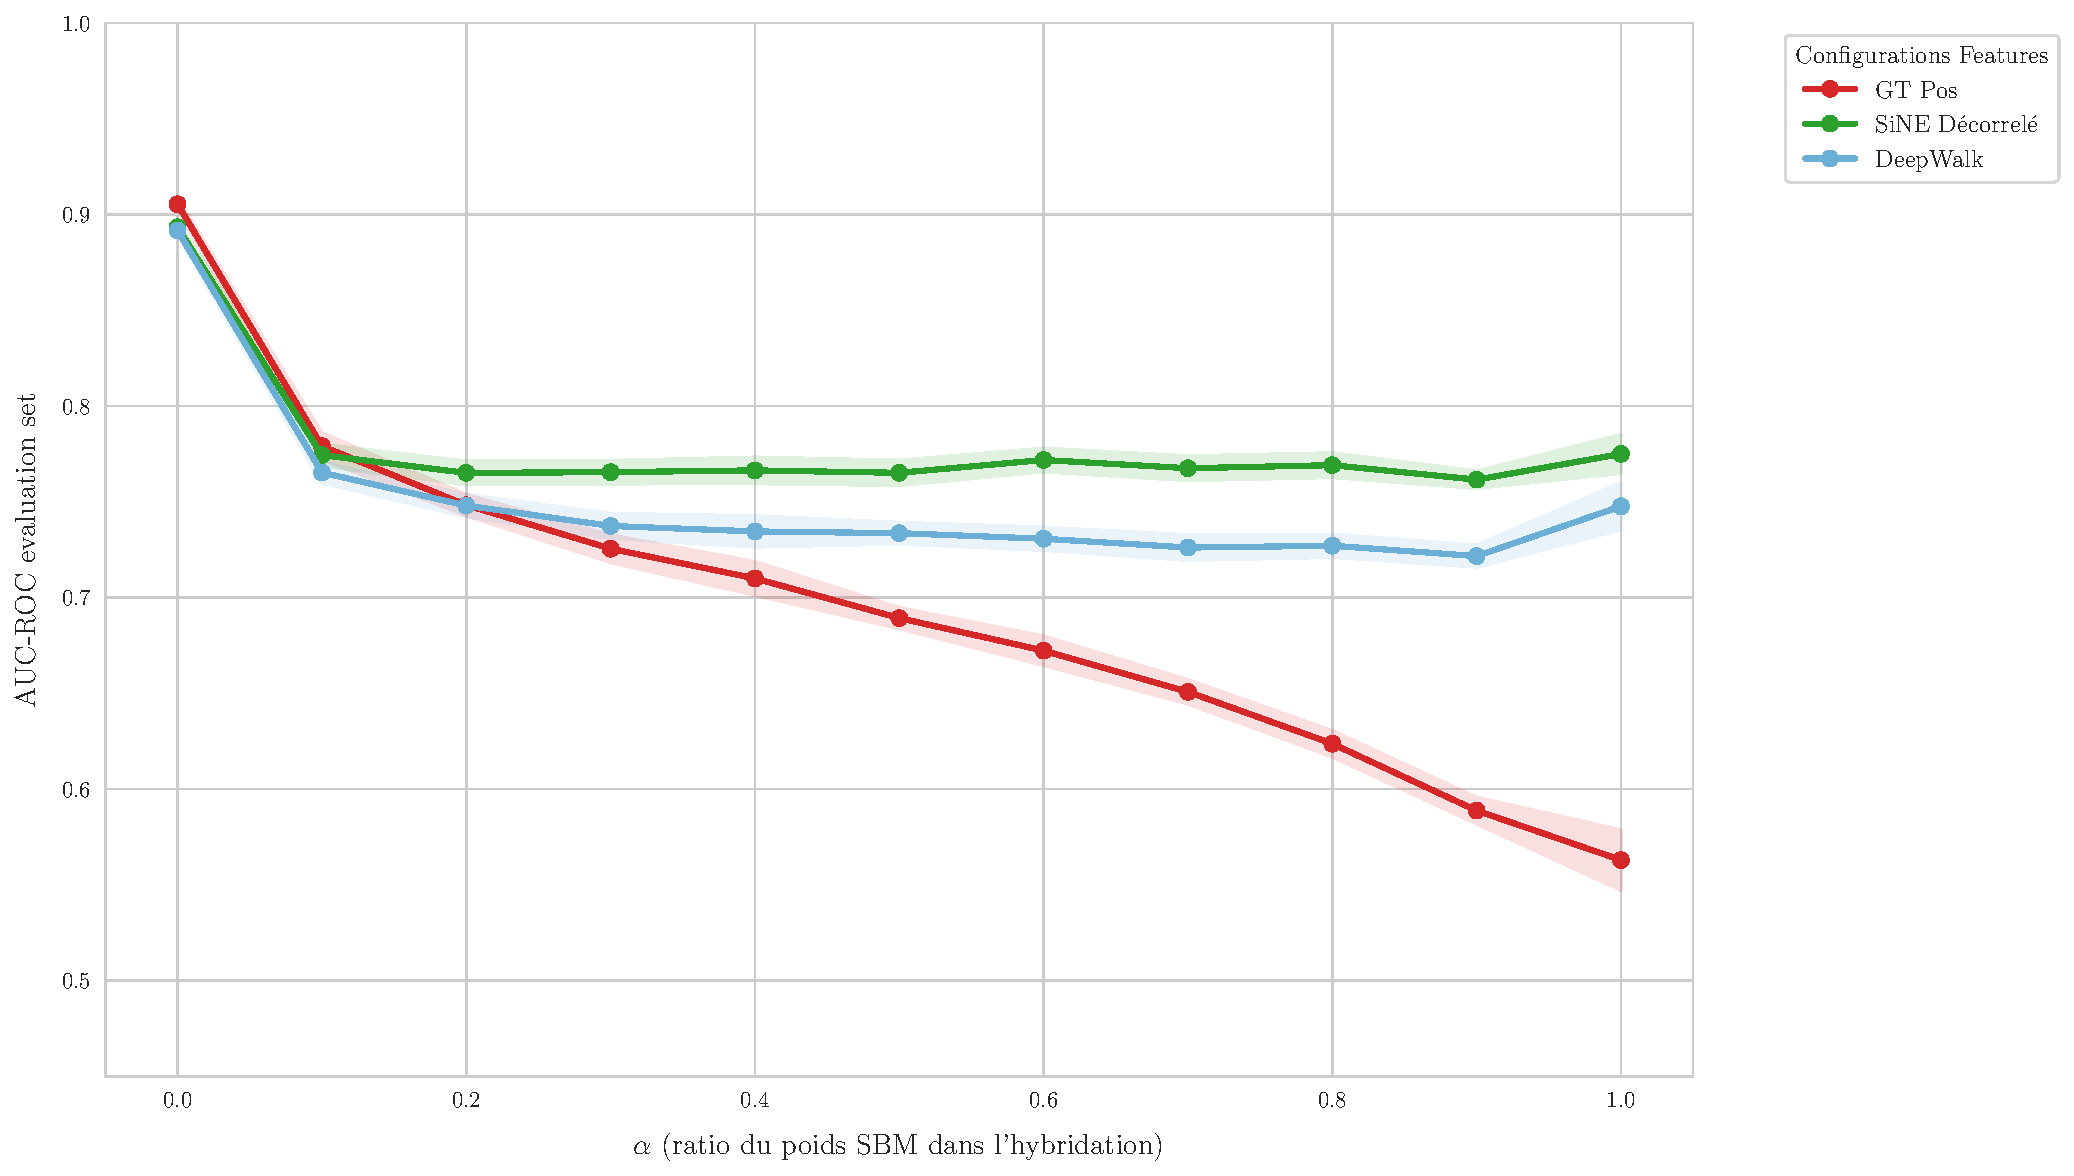
\includegraphics[width=\textwidth]{Plots/212 01_artificial_graphs_shuffled_v6_comuAndEmb_30iter_GTposAndSine_20260529_AUC-ROC_eval_CI99_SBM_ratio.pdf}
        \caption{(d) DeepWalk vs SiNE Décorrélée (hybridation exponentielle)}
        \label{fig:10.4}
    \end{minipage}

    % Légende générale requise par Springer
    \caption{Evolution de l'AUC-ROC du modèle de prédiction de lien \protect\textit{XGBoost} entraîné à l'aide de le \textit{Ground Truth} spatiale et des features standard ou débiaisées (sur 30 itérations).}
    \label{fig:fig10}
\end{figure}
